\documentclass[10pt,twocolumn,letterpaper]{article}

\usepackage{cvpr}
\usepackage{times}
\usepackage{epsfig}
\usepackage{graphicx}
\usepackage{amsmath}
\usepackage{amssymb}
\usepackage{cite}

% Include other packages here, before hyperref.
\usepackage{booktabs}
\usepackage{enumitem}
\usepackage{microtype}

\usepackage[breaklinks=true,bookmarks=false]{hyperref}

\cvprfinalcopy % final submission: removes the review ruler

\begin{document}

%%%%%%%%% TITLE
\title{Instance-Centric Robotic Grasping with ICGNet:\\ A Simulation Study}

\author{
\begin{tabular}{c@{\hskip 1.2cm}c}
Fabio Veroli & Ivan Necerini\\
 s336301 &  s345147\\
{\tt\small s336301@studenti.polito.it} & {\tt\small s345147@studenti.polito.it}\\[6pt]
Alberto Giunti & Jacopo Rialti\\
 s336374 & s346357\\
{\tt\small s336374@studenti.polito.it} & {\tt\small s346357@studenti.polito.it}
\end{tabular}\\[8pt]
Politecnico di Torino
}

\maketitle

%%%%%%%%% ABSTRACT
\begin{abstract}
We integrate ICGNet~\cite{zurbrugger2024icgnet} into a ROS2 pick-and-place system in
Gazebo Sim Fortress (DART physics), coupling its joint instance segmentation, semantic
classification, and 6-DoF grasp predictions with a Franka Panda arm and
MoveIt2~\cite{coleman2015reducing} for \emph{target-driven} grasping: the operator
specifies a semantic class and the robot picks all matching instances into a bin.
Across 180 single-object trials, overall GSR is 32.8\% (90\% on cans). Multi-object
scenes are severely limited by ICGNet's Mask3D failing to generalize from its
TSDF-based training distribution to single-view depth input.
\end{abstract}

%-------------------------------------------------------------------------
\section{Introduction}
\label{sec:intro}

Picking specific objects from cluttered scenes requires simultaneous instance localization,
semantic classification, and 6-DoF grasp computation. ICGNet~\cite{zurbrugger2024icgnet}
addresses this with a single unified architecture: given one point cloud it jointly segments
object instances via Mask3D-style query refinement, classifies each semantically, reconstructs
its 3D shape, and predicts grasp poses with quality scores and gripper widths.

In this work, we integrate ICGNet into a complete ROS2 manipulation pipeline and exploit
this joint output for \emph{target-driven} pick-and-place: the system grasps only instances
of a commanded semantic class, ignoring all others---a direction identified as future work
in the original paper~\cite{zurbrugger2024icgnet}. Figure~\ref{fig:overview} illustrates
the ICGNet architecture.

\begin{figure*}[t]
\centering

\includegraphics[width=0.88\linewidth]{images/mainfig_no_obj_grasps.pdf}
\caption{\textbf{ICGNet Architecture~\cite{zurbrugger2024icgnet}.} Sparse surface and dense
  volumetric features are extracted at multiple scales from the input point cloud.
  Masked-attention instance query refinement decomposes the scene into individually labeled
  instances. Per-instance decoders predict 3D occupancy and 6-DoF grasp affordances with
  quality scores and gripper widths.}
\label{fig:overview}
\end{figure*}

%-------------------------------------------------------------------------
\section{Project Architecture \& Environment}
\label{sec:arch}

\noindent\textbf{Simulation.}
The environment runs in \textbf{Gazebo Sim Fortress} (gz-sim~6) with the \textbf{DART}
physics engine, enabling accurate contact and friction simulation without artificial
object attachment.

\noindent\textbf{Robot and controllers.}
The manipulator is a \textbf{Franka Emika Panda} 7-DoF arm with a parallel-jaw gripper,
integrated via \texttt{gz\_ros2\_control}. The arm uses a \texttt{JointTrajectoryController}
with a \emph{position} command interface; DART handles dynamics internally.
The gripper uses an \emph{effort} interface with a PD controller
($k_p{=}3000$, $k_d{=}20$, $k_i{=}0$) to sustain gripping force on contact.

\noindent\textbf{Motion planning.}
\textbf{MoveIt2}~\cite{coleman2015reducing} plans trajectories via the \texttt{pymoveit2}
client, using \textbf{pick\_ik} for inverse kinematics and \textbf{OMPL
RRTConnect}~\cite{kuffner2000rrt} for motion planning.

\noindent\textbf{Perception.}
An RGB-D camera (640$\times$480, ${\approx}$60$^{\circ}$ HFOV) bridges point clouds to ROS2.
The \texttt{ICGNetGraspNode} exposes \texttt{/icgnet/compute\_grasps}; on each call it runs
inference and publishes per-instance convex-hull \texttt{CollisionObject}s into the MoveIt2
planning scene.

\noindent\textbf{Setup differences vs.\ the paper.}
Table~\ref{tab:diff} highlights the key differences. The most critical is the point cloud
source: the paper trains on TSDF-fused multi-view reconstructions, while we feed raw
single-view Gazebo depth. This mismatch is the primary driver of the limitations discussed
in Sections~\ref{sec:results} and~\ref{sec:multi}.

\begin{table}[ht]
\vspace{-4pt}
\centering
\footnotesize
\setlength{\tabcolsep}{4pt}
\caption{ICGNet paper setup vs.\ our integration.}
\label{tab:diff}
\begin{tabular}{@{}lp{1.55cm}p{1.85cm}@{}}
\toprule
\textbf{Aspect}     & \textbf{Paper}          & \textbf{Ours} \\
\midrule
Point cloud         & TSDF multi-view         & Single-view depth \\
Simulator           & PyBullet                & Gazebo / DART \\
Object dataset      & VGN (343 objects)       & Gazebo DB + primitives \\
Voxel size          & 2\,mm                   & 3\,mm \\
Grasp score thr.    & 0.3                     & 0.0 (executor ranked) \\
Arm execution       & Free-floating gripper   & Panda + MoveIt2 \\
\bottomrule
\end{tabular}
\vspace{-4pt}
\end{table}

\noindent\textbf{Computational graph.}
Figure~\ref{fig:rosgraph} shows the full node topology. All four custom nodes are
highlighted in orange: \texttt{icgnet\_grasp\_node} (inference), \texttt{grasp\_executor\_node}
(pick-and-place FSM), \texttt{scene\_manager} (multi-object scene control), and
\texttt{scene\_visualizer} (live RViz mesh mirror).

\begin{figure*}[t]
\centering
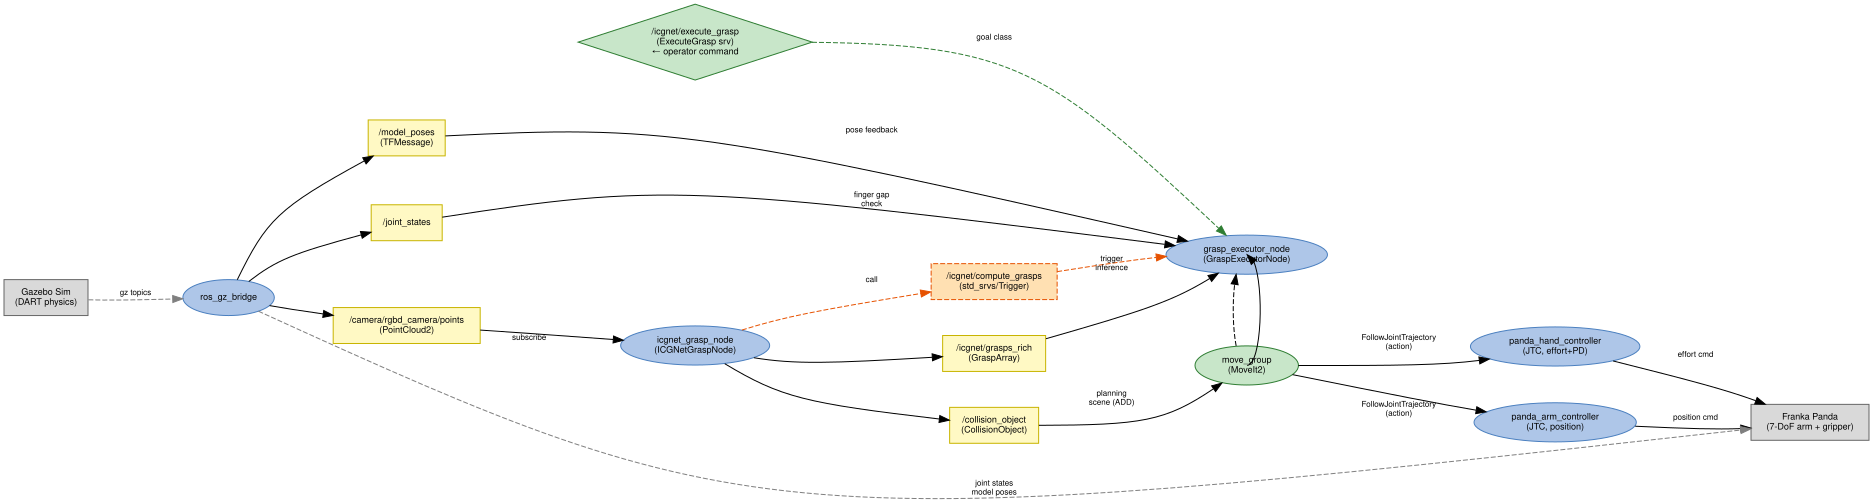
\includegraphics[width=0.90\linewidth]{images/ros2_graph.pdf}
\caption{\textbf{ROS2 computational graph.} Ellipses = nodes (blue = custom, green = MoveIt2);
  yellow = topics; orange dashed = services; green diamond = operator entry point.}
\label{fig:rosgraph}
\end{figure*}

%-------------------------------------------------------------------------
\section{Objective \& Proposed Solution}
\label{sec:obj}

Our goal is to exploit ICGNet's joint output---instance ID, semantic class, and grasp
pose---for \emph{target-driven pick-and-place into a bin}: given a class command
(\eg\ \texttt{"can"}), the system picks all instances of that class and ignores the rest.
This is realized via a ROS2 \texttt{ExecuteGrasp} service whose \texttt{target} field
accepts one of seven class keywords (\texttt{mug}, \texttt{box}, \texttt{can},
\texttt{bottle}, \texttt{cylindric}, \texttt{ball}, \texttt{other}).
No natural-language parser is implemented; the seven class keywords ground the operator intent.

%-------------------------------------------------------------------------
\section{Pick-and-Place Pipeline}
\label{sec:pipeline}

After homing and opening the gripper to clear the camera FOV, the executor calls
\texttt{/icgnet/compute\_grasps}. ICGNet populates the MoveIt2 scene with per-instance
collision objects. Proposals are filtered by width ($\leq$80\,mm), workspace bounds,
target class, and minimum height, then ranked by score. For each candidate (up to five
per run), the following grasp sequence executes:
\begin{enumerate}[noitemsep, topsep=2pt, leftmargin=*]
  \item \textbf{Pre-grasp}: joint-space to 0.12\,m standoff along $\hat{n}$; 180$^{\circ}$ wrist flip as IK fallback.
  \item \textbf{Approach}: Cartesian to $\mathbf{p}_c{=}\mathbf{p}_{\mathrm{tcp}}{+}0.045\hat{n}$ (CO removed to avoid self-collision).
  \item \textbf{Grasp}: gripper closes; gap verified ($5\text{--}40$\,mm); DART friction holds object.
  \item \textbf{Lift}: Cartesian straight-up 0.18\,m.
  \item \textbf{Transfer \& place}: joint-space to bin, Cartesian descent, gripper release,
        retraction to home.
\end{enumerate}
On failure, the object is restored to its inferred pose and the next candidate is tried.

%-------------------------------------------------------------------------
\section{Validation: Single-Object Picking}
\label{sec:results}

We evaluated on 180 single-object trials (6 classes $\times$ 30 runs), one object per trial
with its ground-truth class issued as the target. Table~\ref{tab:gsr} reports the results.

\begin{table}[ht]
\vspace{-4pt}
\centering
\footnotesize
\setlength{\tabcolsep}{5pt}
\caption{Single-object GSR by class (30 trials each, target mode).}
\label{tab:gsr}
\begin{tabular}{@{}lcc@{}}
\toprule
\textbf{Class}   & \textbf{GSR}    & \textbf{Primary failure} \\
\midrule
can              & 90.0\%          & --- \\
box              & 66.7\%          & \textsc{pregrasp\_plan\_fail} \\
bottle           & 33.3\%          & \textsc{perception\_no\_grasp} \\
cylindric        &  6.7\%          & \textsc{perception\_no\_grasp} \\
mug              &  0.0\%          & \textsc{perception\_no\_grasp} \\
ball             &  0.0\%          & \textsc{pregrasp\_plan\_fail} \\
\midrule
\textbf{Overall} & \textbf{32.8\%} & \\
\bottomrule
\end{tabular}
\vspace{-4pt}
\end{table}

\texttt{target=any} (unfiltered best-score) yielded 0\%---the top-ranked grasp is consistently
unreachable (\textsc{pregrasp\_plan\_fail} in 99\% of runs); class filtering is essential.
Dominant failures: \textsc{perception\_no\_grasp} (72 runs) and \textsc{pregrasp\_plan\_fail}
(43 runs). The per-class gap tracks the domain mismatch in Table~\ref{tab:diff}: \texttt{can}
(simple cylinder, well-represented in the VGN set~\cite{breyer2021vgn}) reaches 90\%, while
\texttt{mug} and \texttt{ball} are misclassified even as lone objects---a single-object
symptom of the multi-object failure in Section~\ref{sec:multi}.

%-------------------------------------------------------------------------
\section{Multi-Object Case \& Limitations}
\label{sec:multi}

We implemented a multi-object sweep (\texttt{scene\_manager} + \texttt{\_execute\_sweep}):
targets are spawned alongside distractors, ICGNet is called once per sweep, and
target-class instances are grasped sequentially. The pipeline failed systematically:
ICGNet's Mask3D component does not generalize to multi-object input.
Two failure patterns emerged: \emph{under-segmentation}---multiple objects collapse into
one instance spanning the whole scene, making targeted picking unreliable---and
\emph{over-segmentation with hallucination}---one object splits into multiple instances
with spurious labels (\eg, three objects yielded six predictions including two ``ball''
labels with no ball present).
Ablation of four variables (camera intrinsics, viewpoint, spacing, and object geometry
tested with in-distribution Google Scanned Objects) ruled all of them out.
The sole remaining difference (Table~\ref{tab:diff}) is the \textbf{point cloud pipeline}:
the paper trains on TSDF-fused multi-view reconstructions; we supply raw single-view depth.

%-------------------------------------------------------------------------
\section*{Declarations}

\noindent\textbf{Author Contributions.}
\textbf{F.\ Veroli}: simulation environment (Gazebo/DART, gz\_ros2\_control, camera/TF).
\textbf{I.\ Necerini}: ICGNet inference integration (\texttt{grasp\_service\_node},
point cloud preprocessing, collision-object publishing).
\textbf{A.\ Giunti}: grasp executor state machine, MoveIt2 planning (pick\_ik, RRTConnect),
bin placement logic.
\textbf{J.\ Rialti}: evaluation harness, all trials, ICGNet diagnostic analysis.

\smallskip
\noindent\textbf{Use of Large Language Models.}
LLMs assisted with debugging execution failures and environment setup.
All design, implementation, experiments, and analysis are the authors' own work.

%-------------------------------------------------------------------------
{\small
\bibliographystyle{ieee_fullname}
\bibliography{egbib}
}

\end{document}
